\section{Introducción}

Las redes de monitoreo de calidad del aire de alta densidad son una necesidad creciente de las áreas urbanizadas. Estas permiten monitorear la calidad del aire a escala local, generando información vital para la toma de desiciones en áreas de salud pública. Al incrementar la cantidad de estaciones de monitoreo, la resolución de los datos aumenta, pero también aumentan el costo, la infraestructura y el personal necesario para atenderlas\cite{urban_air_quality}. De la misma forma, la demanda para redes de monitoreo climatológico de alta densidad ha ido en aumento por su utilidad en la medición de los impactos de las políticas de control en el ambiente\cite{muller_sensors_and_the_city}.

Las instalaciones de monitoreo meteorológico eran acostumbradas a ubicarse en las afueras de complejos ubranizados, centrados en la recolección de información para un análisis a escala global de los datos climatológicos, tales como el análisis del calentamiento global y los índices de radiación, así como otros datos importantes. Debido a los cambios en las necesidades de calidad y cantidad de datos, esto ha cambiado significativamente\cite{oke_2004}.

Las estaciones de monitoreo climatológico funcionan de la misma forma que la mayoría de los servidores en el mercado; Un equipo de cómputo que está corriendo un servicio escucha constantemente las peticiones de los clientes a los que está conectado, creando y actualizando datos conforme es necesario. El equipo de cómputo además se conecta a sensores que utiliza para el monitoreo contínuo de datos, los procesa, y los almacena para su posterior análisis. Esto, crea la posibilidad de integrar y crear sistemas de monitoreo de equipos de cómputo para el monitoreo de la salud de las estaciones

\section{Planteamiento del problema}

\subsection{Antecedentes}

El desplegar y mantener una red meteorológica compone bastantes retos, entre ellos está la  esto aunado a

\cite{rpi_weataher_station}

Con la creciente importancia de los datos meteorológicos fidedignos, es importante la creación y mantenimiento de redes meteorológicas de alta densidad para el monitoreo climatológico de áreas urbanas y conurbanas.


Pero de la misma forma, al ser un equipo de cómputo con funciones específicas, requiere de un alto grado de entendimiento de las funciones que realiza para poder modificarlas, así como un diagnóstico detallado y complicado para poder repararlas en caso de un fallo.

[...] Párrafo sobre los problemas de escalabilidad de las estaciones [...]. *No es posible crear una red de estaciones y mantenerlas y monitorearlas sin esfuerzo*.

[...] Párrafo puente pendiente [...]

Por lo tanto, se propone la creación de un servicio e interfaz para facilitar la administración y mantenimiento general de los equipos meteorológicos, que *has an objective to aim to a broader audience* para así reducir a los tiempos de respuesta de los fallos de las estaciones meteorológicas.

> Importancia de los datos meteoroleogicos

> Redes meteorológicas de alta densidad



Debido a la *[disponibilidad e integridad]* de los datos requerida en las estaciones meteorológicas, han buscado crear redes resilentes [...], pero eso no evita que sean completamente resistente a fallos.

Actualmente las estaciones funcionan [...].

> Nagios
Sin embargo, la complejidad de la red meteorológica crece considerablemente cuando se toma en cuenta que las estaciones meteorológicas varían

\begin{figure}[!ht]
	\centering
	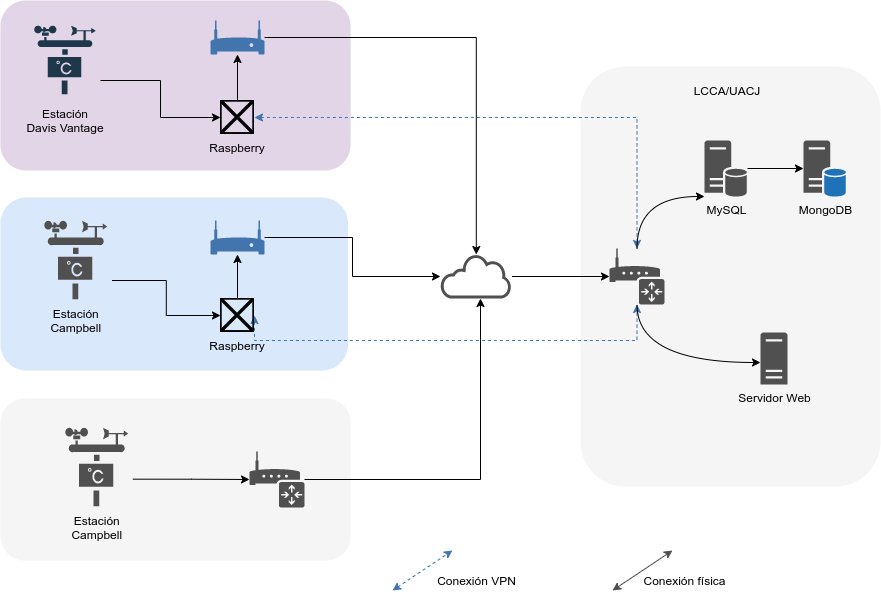
\includegraphics[width=.80\linewidth]{images/diagrams/current_network.png}
	\caption{Diagrama del protocolo REST.}
	\label{fig:current_network}
\end{figure}

\subsection{Definición del problema}

La falta de una plataforma estandarizada para el monitoreo de las estaciones meteorológicas independiente de las compañías crea un problema de
\cite{muller_sensors_and_the_city}

Debido a la complejidad de los sistemas de monitoreo tecnológico, y al alto grado de conocimiento que es requerido para el monitorear las estaciones y darles mantenimiento. [...] el atender los fallos de las estaciones meteorológicas lleva tiempo y expertise, aún cuando estas fallas no sean críticas o complicadas

\cite{red_climatologica_uacj}

Fácil, entendible, UX/UI.

%! Tiempo de respuesta como aporte secundario a la metodología
